\date{\vspace*{-0.2in}}

%%%\renewcommand{\baselinestretch}{2}
\documentclass[10pt]{sigplanconf}
\nocaptionrule


\newcommand{\footnotenonumber}[1]{{\def\thempfn{}\footnotetext{\small #1}}}
\usepackage[normalem]{ulem}
\usepackage{graphicx}
\usepackage{times}
\usepackage{subfigure}
\usepackage{url}
\urlstyle{rm}

\usepackage{color}
\usepackage{listings}
\usepackage{amsmath}
\usepackage{amsfonts}
\usepackage{amssymb}
\usepackage{comment} 
\usepackage{setspace}
\singlespacing
%\onehalfspacing
\newtheorem{thm}{Theorem}
\newtheorem{prop}[thm]{Proposition}
\newtheorem{cor}[thm]{Corollary}
\newtheorem{lem}[thm]{Lemma}
\newtheorem{defn}[thm]{Definition}


\newcommand{\cfunction}[1]{{\bf \tt #1}}
\newcommand{\malloc}{\cfunction{malloc}}
\newcommand{\realloc}{\cfunction{realloc}}
\newcommand{\free}{\cfunction{free}}
\newcommand{\madvise}{\cfunction{madvise}}
\newcommand{\brk}{\cfunction{brk}}
\newcommand{\sbrk}{\cfunction{sbrk}}
\newcommand{\mmap}{\cfunction{mmap}}
\newcommand{\munmap}{\cfunction{munmap}}
\newcommand{\mprotect}{\cfunction{mprotect}}
\newcommand{\mlock}{\cfunction{mlock}}

\hyphenation{app-li-ca-tion}
\hyphenation{Die-Hard}
\hyphenation{Archi-pe-la-go}
\hyphenation{buf-fer}

\lstset{language=c++, basicstyle=\small\ttfamily,frame=single,tabsize=4}

\definecolor{Gray}{cmyk}{0,0,0,0.5}

\begin{document}

%\renewcommand{\baselinestretch}{2}

\conferenceinfo{XXXXXXXXXXXXXXXXXXX}

\title{Sheriff: Detecting and Eliminating False Sharing}

\authorinfo{}

%Tongping~Liu \and Emery~D.~Berger}
%{Dept.\ of Computer Science \\ University of Massachusetts, Amherst \\
%Amherst, MA 01003} {\{tonyliu,emery\}@cs.umass.edu}

\maketitle

\begin{comment}
%%%%%%%%%%%%%%%%%%%%%%%%%%%%%%%%%%%%%%%%%%%%%%%%%%%%%%%%%%%%%%%%%%%%%%%%%%%%%%%%%%%%%%%%%%%%%
Story:
Multi-core processors or NUMA are now widely used in order to avoid the physical limits of hardware. 
Multi-threaded is considered as one way to take full advantage of those computation resources. Unfornately, 
writing efficient multi-threaded program is not an easy task; 
false sharing problem can reduce the performance greatly, 
even worse, one program with serious false sharing problem can run slower on multi-core machine that that on 
on single-core machine with the same cpu frequency of every core.

This paper presents Sheriff, a system to detect those false sharing problem in multi-threaded c/c++ programs. 
Comparing to previous tool, Sheriff has a very low performance overhead, 
averagely the performance overhead is about 15\% in our experiments. 
For most programs, Sheriff can run almost the same speed or even faster than original program
using pthreads library. 
The second advantage of Sheriff is that there is no false positives at all. 
The false sharing problems reported by Sheriff are actual false sharing problems.

The third adanvatage of Sheriff is that Sheriff can pinpoint the code to cause the false sharing problems. 
For heap objects, Sheriff can point out the allocation site, 
then it is easy for programmer to fix the false sharing problem given the callsite information,
even for some one that are not familiar with the code. 
For global objects, Sheriff can point out those objects' name and length information which has false sharing problem.

How Sheriff to do that?
First, we are using a runtime system which maintains the semantics of multi-threaded program.
To detect those modifications by different threads, we turn those multi-threaded program into a 
multi-process program and use the page protection mechanism to capture those writes on different threads.
In order to capture those writes of different memory, we introduce a "twin" page in the page fault handler;
then we utilize the lazy differentiating mechanism (which has been widely used in distributed share memory) to 
find acutal writes in each phase. 
In order to capture those cache invalidation of different threads, we maintain a global array which is used to
maintain the last thread id to write on one cache line. We use a 
conservative mechanism to count those invalidation of cache lines, 
only those interleaving writes by different threads are counted as an invalidation of corresponding cache line. 
In order to differentiate the false sharing problem from true sharing problem, 
we also keep a word-based version number array 
which is used to record every writes information on each word, including thread id and version. (We use a special
id to identify multi-threads on one word).
 
Also, this word-based versioning mechanism
can help us to the precisely locate the object that are causing the problem if multiple objects are located in 
the same physical cache line.

In order to catch those false sharing problem caused by long transaction, 
we introduce one "sampling mechanism" which can get continutive writes of different threads.

In order to pingpoint the allocation site, we will attach the callsite information for those allocation. Then we can present those callsite when we find out much invalidation. 
 
What else Sheriff can do?
First, Sheriff can work as a run-time system, which can tolerate some of the false sharing problems. 
Second, Sheriff can work as a system which can detect those race condition problems undetectable using those lock-set based tool.
Third, Sheriff can also work as a system to tolerate race problem, like Isolator.

Future work:
(1) Pinpoint the line number to access the cache line by using the "watch point" technique.
(2) Figure out the problem caused by read-write false sharing problem by using the "watch point" technique.
(3) Design a run-time system which can tolerate the false sharing problem in a very low overhead. Profiling 
on specified input should be very helpful to find the problem.
%%%%%%%%%%%%%%%%%%%%%%%%%%%%%%%%%%%%%%%%%%%%%%%%%%%%%%%%%%%%%%%%%%%%%%%%%%%%%%%%%%%%%%%%%%%%%
\end{comment}

\begin{abstract}
%How is existing work?
%Sharing inside mulithreaading programs is not easy, they can easily cause correctness or performance problem. 
%Inappropriate sharing can dramatically degrade the performance of 
%mulithreading programs and seriously affect the scalability. 
%So detecting false sharing accurately and precisely can be helpful for user to fix corresponding performance problem. 

\begin{comment}
False sharing is notorious for performance degradation in multithreaded
programs. It apprears when two or more threads running on different cores periodically access 
different portions of data that can fit into one cache line. Since caching
system in a multicore processor needs to ensure a coherent view of memory
accross all cores, it has to grant an exclusive access
for each write operation by invidating duplicate copies in other cores. As a
result, frequent cache invalidation can seriously affect the scalability and
performance of multithreaded programs.
\end{comment} 

False sharing is a notorious performance issue for different software stacks, 
which can dramatically degrade the performance and seriously affect the scalability of 
systems.

%Many reserach efforts have been made to detect false sharing. 
Unfortunately, previous approaches to detect false sharing
either introduce significant performance overhead, or fail
to report false sharing accurately and precisely, or have different limitations of usage. 
%\sheriff{}, the prior state-of-the-art tool, 
%can only detect write-write false sharing in applications using \pthreads{} library.
This paper presents a novel approach, \Predator{}, to combine compiler instrumentation
and runtime system to detect false sharing. 
%the compiler instruments every memory access and 
%the runtime system collects and analyzes memory accesses to detect false sharing problems.
Since it does not rely on any hardware, OS or threading library, this approach can be
applied to the entire software stack without any limitation. 
\Predator{} can detect false sharing accurately and precisely: it reports no 
false positives and pinpoints exact objects with false sharing problems.
%Also, unlike previous work, this method can be extended to
%identify false sharing problems across the entire software stack, including 
%hypervisors, operating systems, libraries and applications. 
Experimental results on two popular benchmark suites 
show that \Predator{} not only detected all known false sharing problems but also revealed 
two unknown false sharing problems.
Besides, \Predator{} have successfully detected false sharing of real applications,
including \texttt{mysql} server application and \texttt{boost} library. Fixing these
false sharing problems improves performance by $6\times$ and $40\%$ correspondingly.

Moreover, existing tools can only detect those manifested false sharing problems.
However, occurrences of false sharing can be affected by alignments between
objects and cache lines: any change of compiler optimization, compiler, memory manager, 
memory allocation order, cache line size or different target binary 
may change alignments, and thus affect occurrences of false sharing, 
which leaves many of them undetected by existing tools.
\Predator{} is the first tool which can accurately predict possible false sharing 
without the need of occurrences. 
It can report all false sharing problems with only one execution and with reasonable overhead, 
around $6.7\times$ performance overhead on average.

%What is novel in our work?
%How is the performance overhead?

\end{abstract}

\terms
Performance, False sharing

\keywords
Concurrency, False Sharing, Performance, Multi-threaded program

%%%%%%%%%%%%%%%%%%%%%%%%%%%%%%%%%%%%%%%%%%%%%%%%%%%%%%%%%%%%%%%%%%%%%%%%%%%%%%%%%%%%%%%%%%%%%
%%%%%%%%%%%%%%%%%%%%%%%%%%%%%%%%%%%%%%%%%%%%%%%%%%%%%%%%%%%%%%%%%%%%%%%%%%%%%%%%%%%%%%%%%%%%%

\section{Introduction}
%False sharing problem is a cache usage problem. 
%Cache, with much faster access speed than main memory, is normally utilized by CPU
%to accelerate program executions by preloading a fixed size of data into the cache each time, 
%called as a cache line.  

%%%%%%%%%%%%%%%%%%%%%%%%%%%%%%%%%%%%%%%%
% Why 
%%%%%%%%%%%%%%%%%%%%%%%%%%%%%%%%%%%%%%%%
\label{sec:intro} 
False sharing is notorious for performance degradation in multithreaded
programs due to cache coherence protocol, which exists in most mordern 
 mutlicore processors.
The reason of having cache coherence protocol is to ensure the correctness of
program executions: 
if some cache line data on a core needs to be updated, the duplicated data in any other core's private 
cache must be invalidated at cache-line level (e.g., 64 Bytes). 
However, frequent invalidations can cause severe performance problem.
In the case of false sharing where multiple threads access different locations
in the same cache line in a \textit{ping-pong} manner, generated cache
invalidations can easily degrade program performance as much as an order of magnitude. 
%Because cache invalidation can cause a thread accessing the same cache line to stall and wait for the data 
%to be loaded from main memory, wasting both the CPU time and memory bandwidth in the same time. 
Unfortunately, the hardware evolution is on the venue of building more cores
with larger cache line size, which makes false sharing increasingly common.

Prior studies have shown that false sharing affects different levels of current software stack.
It has been found in OS (Linux kernel~\cite{OSfalsesharing}), Java virtual machine~\cite{JVMfalsesharing}, 
common libraries~\cite{libfalsesharing} and real applications~\cite{appfalsesharing, mysql}. 
People also observed false sharing in runtime system such as share memory system
~\cite{dsmfalsesharing} and transactional memory ~\cite{tmfalsesharing}.
Although many efforts have been made in false sharing detection, existing
tools have various limitations:
they either introduce significant performance overhead~
\cite{falseshare:simulator, falseshare:binaryinstrumentation1,falseshare:binaryinstrumentation2}, or 
 are incapable of reporting false sharing 
precisely and accurately~\cite{qinzhaodetection, detect:ptu, detect:intel, falseshare:binaryinstrumentation1, DProf, falseshare:binaryinstrumentation2}, 
or require special OS support~\cite{OSdetection}.
% or they can only detect one kind of
%false sharing problem on a specific multithreading library~\cite{sheriff}.
The state-of-the-art tool, Sheriff~\cite{sheriff} overcomes these limitations. However, 
it can only detect write-write type false sharing in programs using pthreads library,
and can not work correctly on programs using ad-hoc synchronizations or using stack variables to 
communicate among different threads. Also, to the best of our knowledge, none of them has been 
utilized to find false sharing problem in real applications.

Despite their different features and limitations, all existing detection tools 
have two common drawbacks.
The first drawback is that existing techniques can not detect false sharing for 
the entire software stack, whereas they can work on a specific level of software stack.
The second drawback is that they can only detect those false sharing occurring in current execution.
However, as pointed out by Nanavati et al.~\cite{OSdetection}, 
some dynamic properties of a system can easily 
change the manifest of false sharing problems. They also give an example that 
{\it "GCC fixes false sharing in the Phoenix linear\_regression benchmark 
at -O2 and -O3 optimization, while clang fails to even at the highest
optimization level".}
To our understanding, those dynamic properties include 
choosing different compiler, 
enabling different compiler optimizations, 
using different memory management schemes,
and changing different target platforms such as address mode (32-bit or 64-bit) and cache line
size (64 Bytes or 128 Bytes) and so on. Unfortuantely, 
existing detection tools do not consider these dynamic properties, and
therefore are unable to identify potential performance-degrading false
sharing problems that may occur in an execution under a set of different 
dynamic properties.

In this paper, we propose a new false sharing detector, \defaults{}, aiming to
not only {\it detect} all existing false sharing problems accurately and precisely,
but {\it predict} those potential 
false sharing problems that may appear in a slightly different environment. 
%To be more specific, 
%\defaults{} can report potential false sharing problems with different cache line size and different starting address of an object 
%without the need of another execution. 

\Defaults{} has the following contributions:
\begin{itemize}
\item
% methodology
\defaults{} provides a novel false sharing detection method by
combining compiler instrumentation with runtime system.
%, which can avoid the shortcomings of existing tools. 
Since \defaults{} neither relies on the support of specific hardware and OS ,
nor binds to specific threading library, 
it is suitable for the entire software stack, 
i.e., hypervisors, operating systems, libraries and applications. 
%Since compiler can be utilized to do selective instrumentation, 
%\defaults{} can be utilized to detect all kinds of false sharing problem with ideal overhead. 

% effect: can detect all kinds of false sharing problems.
\item
\defaults{} can actually detect all kinds of false sharing problems accurately and precisely 
with reasonable overhead. 
It reveals some unknown false sharing problems in those benchmark suites evaluated by 
previous approaches.
It is also the first tool to detect false sharing problems existing in real applications, e.g.,
\texttt{mysql} server application and \texttt{boost} library.
% combine compiler instrumentation with runtime system, so that it can 
%detect all kinds of false sharing problem including write-write false sharing. 
%avoid the shortcomings of runtime-only system, where Sheriff can not detect the read-writee false sharings. 
%Also, because of the limit of their implementation, Sheriff can not support the program using the ad hoc synchronization
%or using the stack variables to communicate among different threads.
%Also, it looks like that we can provide a evenly performance overhead.
%Also, sheriff should only work on specific thread library, currently, it can only work on pthreads library. 
%We are trying to extending the same idea to different thread library. Now we can also run DeFault to detect all 
%false sharings using other threads libraries.

% prediction
\item
\defaults{} is the first approach to predict potential false sharing that does
not manifest in an execution but may appear and greatly affect the performance of programs 
in a slightly different environment. 
This avoids the predicament of detection tools: problems may occur in a real
environment rather than test environment due to environmental changes. 
%Existing approaches is based on specific hardware,
%runtime environment(using specific libraries and compilers) and specific cache line size, which is OK to detect those 
%existing false sharings. But they fail to capture those variables or objects which can greately slow down performance 

%In order to save memory usage, we propose a threshold invoked detection based on the predefined number of writes on a cache line, which
%can be used to track the .

\end{itemize}

The orgnization of this paper is as follows .....

%There are two types of false sharings:
%A. Different threads are accessed different locations according to the definition of flase sahrings. 
%B. Locations with a large amount of reads is placed in the cache line with a large amount of writes.
%For the second type, existing tools may tend to miss that.  



\section{Sheriff Overview}
\label{sec:overview}

\DoubleTake{} improves performance for dynamic analysis by utilizing a record-and-replay idea, 
which is discribed in Figure~\ref{fig:overview} {\bf FIGGGURE}.. 
\DoubleTake{} divides an execution of a program into multiple epochs, at the boundaries of irrevocable
system calls (discussed in Section~\ref{sec:syscall}) or different types of exits, e.g., 
segmentation faults, aborts or normal exit.
In the beginning of an epoch, \doubletake{} takes a snapshot of program state, 
including changeable memory and registers.
During an epoch, a program proceeds at full speed with extremely light-weight recording on results of
certain system calls, in order to facilitate re-execution. 
In the end of an epoch, \doubletake{} checks the evidence for errors. 
We have implemented checks for three types of errors (discussed in Section~\ref{sec:applications}), 
including heap buffer overflows, memory usage-after-free errors, and memory leaks. 
If an error is detected, 
\doubletake{} switches to re-execution mode (described in Section~\ref{sec:re-execution}) 
to gather detailed information of the error.
If no error is detected and a program ends this epoch because of an irrevocable system call, 
\doubletake{} will issue the irrevocable system call and start a new epoch.
Because \doubletake{} only check memory errors in the end of epochs and ends epochs rarely, 
which amortizes the cost of checking errors over 
long periods of uninterrupted execution, 
\doubletake{} achieves extremely light performance overhead.

Checking evidence of errors and gathering detailed error information are application specific. 
In order to detect buffer overflows and memory usage-after-free errors, \doubletake{} fills 
memory with canaries, which is discussed in Section~\ref{sec:canaries}.
In order to precisely identifying the instruction reponsible for these two errors, 
\DoubleTake{} installs hardware watch points (see Section~\ref{sec:watchpoints}) before 
actual re-executions. 
In order to reproduce those found memory errors deterministically, 
it is crucial for \doubletake{} to have exactly the same memory allocations in re-executions. 
Because it is difficult to do this in a general memory allocator,
\DoubleTake{} designs its custom memory allocator for all memory allocations and deallocations, 
which is discussed in Section~\ref{sec:allocator}. 

\subsection{System Calls}
\label{sec:syscall}

% Why we need to care about system calls. Because some system calls are irrevocable.
% However, not all IO are irrevocable. For example, if a file reads twice, as long as 
% it returns the same result. We do not need to undone the results of IO operations. 
\doubletake{} ends epochs on irrevocable system calls: the execution before
and after irrecocable system calls belong to different epochs.
Irrevocable here has a different meaning as that in transactional memory programming. 
In transactional memory programming, irrevocable actions include IO and system calls whose
effect cannot be rollbacked or completely invoked in user space~\cite{Irrevocabletrans}.
\doubletake{} relaxes the definition of irrevocable: only the results of system calls cannot be 
reproduced are considering to be irrevocable system calls. 
System calls are classified to the following types.

\begin{table}[t]
	\centering
	\small
	\renewcommand{\arraystretch}{1.5}
	\begin{tabular}{r|p{6cm}}
		\textbf{Category} & \textbf{Functions} \\
		\hline
		
		Repeatable		& \texttt{getpid}, \texttt{sleep}, \texttt{pause}\\
		
		Recordable		& \texttt{mmap}, \texttt{gettimeofday}, \texttt{time}, 
						  \texttt{clone} , \texttt{open}\\
		
		Checkpointed		& \texttt{write}, \texttt{read} \\
		
		Delayed			& \texttt{close}, \texttt{munmap} \\
		
		Irrevocable		& \texttt{fork}, \texttt{exec}, \texttt{exit}, \texttt{lseek}, \texttt{pipe}, \texttt{flock}, \texttt{socket related system calls}\\
	\end{tabular}
	\caption{
		System calls handled by \doubletake{}. Other calls not listed are treated as irrevocable, and will end the current epoch. Section~\ref{sec:syscalls} describes how \doubletake{} handles calls in each category.
		\label{tbl:syscalls}
	}
\end{table}

\label{sec:syscalls}
\paragraph{Repeatable system calls} do not modify system state, and will always return the same result.
This category includes \texttt{sleep}, \texttt{pause}, and system calls to query system's state, e.g. \texttt{getpid()}, \texttt{fstat} and \texttt{stat}. 
\doubletake{} does not need any special handling for these system calls.
	
\paragraph{Recordable system calls} may return different results if they are re-executed. 
\doubletake{} records the result of these system calls. 
During re-execution, \doubletake{} will simply return the saved result 
instead of re-executing the system call. 
This category includes \texttt{mmap()}, \texttt{gettimeofday()}, \texttt{time()}, and \texttt{clone()}.

\paragraph{Checkpointable system calls} modify system state, 
but \doubletake{} can save this state beforehand and restore it prior to re-execution. 
Most of file IO related system calls fall into this category. 
For example, the \texttt{write()} system call can modify the contents of a file and moves the 
file positions inside operating system.
They can be treated as irrevocable system calls, but that can greatly affect performance 
because of intensive usages in applications.
\doubletake{} saves those file positions of openning files in the beginning of each epoch and 
recovers those file positions before re-execution. 
%Because \texttt{read()} and \texttt{write()} can be used in socket communications, which is considered
%as irrevocable system calls, \doubletake{} checks whether those file descriptors are related to 
%actual files. If they are invoked on actual files, there is no other operation on those file related system calls.  
	
\paragraph{Delayable system calls} will irrevocably change program state, but can safely 
be delayed until the end of the current epoch. 
\doubletake{} delays all calls to \texttt{munmap()} and \texttt{close()}.
	
\paragraph{Irrevocable system calls} cannot be replayed. \doubletake{} must end the current epoch 
before these system calls are allowed to proceed. A system call not belonging to previous categories
can be conservatively treated as an irrevocable system call.

\vspace*{\baselineskip} 
During normal execution of an epoch, \doubletake{} intercepts all calls to \pthreads{} 
library functions that may issue system calls. \doubletake{} actually handles much more function calls
than the listed number of system calls. For example, \texttt{open()}, \texttt{fopen()}, \texttt{fdopen}, \texttt{freopen()}, and \texttt{creat()} can possibly call \texttt{open} system calls. 
Then all of these library functions should be intercepted. 
%We assume that other libraries are built 
%on this library: there is no direct system call from other libraries or applications.

To reduce overhead, we should reduce the amount of epochs as much as possible by 
recording, checkpointing and delaying system calls since starting and ending an epoch 
involves large performance overhead, as discussed in Section~\ref{sec:implementation}, 
Currently, \doubletake{} only optimizes those system calls invoked by evaluated applications.
Current category of system calls can be seen in Table~\ref{tbl:syscalls}. Other system calls
not mentioned here belong to the category of irrevocable system calls. 

\begin{comment}
To support multithreading programs, \DoubleTake{} has to record the order of synchronizations 
and replay them in the same order (Section~\ref{sec:multithreading}) and design memory allocator specially (Section~\ref{sec:mtheap}).

The basic idea of \DoubleTake{} is to greatly {\em reduce the number of checkings}:  
instead of checking a possible out-of-bounds error before every memory access, 
\DoubleTake{} checks all possible out-of-bounds errors of the whole program 
before those irrevocable system calls or in the end of an execution.
By checking buffer overflows accumulatively, \DoubleTake{} amortizes 
checking overhead over long executions and achieves much better performance. 
As showed in Figure~\ref{fig:diagram}, if a program does not have buffer overflows, 
it continues to perform those system calls and 
starts a new epoch after them by snapshotting state of this execution. 
If a program is found to have buffer overflows, \DoubleTake{} re-executes it by rolling back 
to last good state after installing hardware watchpoints on those overflowing addresses.
By handling exceptions, 
\DoubleTake{} can pinpoint precisely those memory accesses causing memory overflows without
actually instrumenting every access. 
\end{comment}


\subsection{Canary Mechanism}
\label{sec:canaries}
Canaries, also called as sentinels, are normally put before or after each actual object.
They are initialized to a special value in the beginning so that modifications of those values
indicates the problems.
Canaries have been used by many previous works to
detect buffer overflows ~\cite{overflow:purify, exterminator, overflow:lbc}.
Similarly, \stopgap{} puts canaries before and after heap objects, which can be used .
to detect buffer underflows and overflows.
The size of canary is a balance between memory overhead and precision.
As discusssed by Hasabnis et al. ~\cite{overflow:lbc}, larger size helps to detect more
buffer overflows, but increasing memory overhead.
\stopgap{} chooses the size of a pointer as the size of each word-based canary:
4 bytes for 32 bit binaries and 8 bytes for 64 bit binaries.
For those objects with size not aligned by words, \stopgap{} filles byte-based canaries before a
word-based canary.

\stopgap{} maintains a global bitmap to mark placements of those canaries:
if a word includes canaries, either a word-based canary or multiple
byte-based canaries, its corresponding bit is set to $1$.
Since \stopgap{} only uses a bit for each word, this helps to reduce memory overhead of the bitmap.
Previous works use a bit for each byte in order to capture one-byte buffer overflow~\cite{overflow:lbc, AddressSanitizer}.
However, it is uncessary to do this since \stopgap{} embeds size information of each heap object
into the header, thus by coming with size information and byte-based canaries \stopgap{} doesn't
loose the precision of detecting one-byte buffer overflows.
Reducing the size of bitmap helps improving the speed of heap integrity checking too.

\subsection{Watch Point Mechanism}
\label{sec:watchpoints}
Watch point mechanism relies on hardware debug registers to monitor memory accesses on
specific addresses. Previous work has used this mechanism for their specific 
targets \cite{fastboundschecking, Kivati}.

Debug registers are universally supported by most if not all existing CPUs, such as
X86 and X86-64 architecture, PowerPC, MIPS, ARM, etc. 
The main target of debug registers is to support software debuggers, e.g. gdb. 
In X86 and X86-64 architectures, there are four debug address registers, one debug 
status register and one debug control register. 
A user can set up debug address registers to hold those addresses that want to monitor 
before executions of a program. 
Then this user can be notified by an exception whenever a memory access matches one of those 
debugging address in debug registers. 

%\DoubleTake{} installs the addresses of canaries with buffer overflows and watches memory
%accesses on them in the re-execution phase by handling those exceptions generated by debug registers. 
%By analyzing the context of signal handler, 
%\DoubleTake{} can precisely locate those instructions causing buffer overflows and report to users.
%More implementation details are discussed in Section~\ref{sec:installwatchpoints}. 

\subsection{Customized Heap Allocator}
\label{sec:allocator}
A general memory allocator invokes a big number of \texttt{mmap} or \texttt{sbrk} system calls,
thus it is hard to repeat memory usages of a program without recording all memory allocations. 
%related system calls and repeating
%them in re-execution phase.
\DoubleTake{} utilizes customized memory allocator for its heap allocations to overcome these shortcomings. The memory allocator of \DoubleTake{} is built on Heap Layers ~\cite{heaplayers}, 
%repeat memory allocations in re-execution phase.

%However, it is normally impossible to do this for multithreading programs.
\DoubleTake{} pre-allocates a fixed size of memory 
from its underlying operating system using \texttt{mmap} system calls and 
satisfies memory allocations from this block of memory.
All heap objects has the size of {\it power of $2$}, known as block size. 
When an object is allocated, \doubletake{} adds a object header to each object, including block size,
actual object size and canary.
When an object is deallocated, it is put into a corresponding free list of the memory allocator, 
holding objects with the same block size. 
\DoubleTake{} never changes size of an object so there is no split and merge operation on heap objects.
If size of an allocation is less than {\it power of 2}, 
\DoubleTake{} allocates an object with the size of next {\it power of 2}.
% but putting canaries
%right after this actual object in order to detect .
%The support for multithreading programs can be seen in Section~\ref{sec:mtheap}.

% why it is deterministic?
Since it is conventient to find out memory usage conditions in the beginning of each epoch 
and all memory allocation are deterministic according to the order of program execution from the same heap without involving other system calls,  
it is relatively easy to reproduce memory usage in production runs.
% Because of this design, it is convenient to take a snapshot in production runs 
%and repeat memory usage in reproduction runs. 




\section{Simulation of multi-threaded program}
\label{sec:simulation}

This section we are going to talk how to replace threads with processes while still maintain
the same semantics of multithreaded program.

We are going to answer the following questions in the following subsections:
\begin{itemize}
\item How to turn threads into proceses? 
\item How to maintain the semantics to share the same address space?
\item How to share file access?
\item How to handle synchronization among threads?
\end{itemize} 

In the end, we are going to talk how to simuate the threads in one phase.
\subsection{Thread Creation and Exit}
Sheriff intercepts those function calls of \texttt{pthread\_create()} then replaced that with a \texttt{fork()} system call.
Child processes invokes the routine passed by \texttt{pthread\_create()} calls. 
In this way, Sheriff fork off new processes instead. 

Sheriff use one explicit \texttt{\_exit()} call to terminal current thread.

\subsection{Share Address Space}
\label{simulation:sharememory}
In order to create the illusion of multi-threaded programs that 
different threads are sharing the same address space, 
Sheriff uses the memory mapped files to share the heap and globals across different processes.
It is noted that Sheriff don't try to share the stack across different processes 
because different threads have their own stacks and 
it is un-common to use stack to communicate between different threads.

Sheriff creates two different mappings for both the heap and the globals. 
One is shared mapping, which is working as a backstore using to hold those shared state. 
Another one is private, copy-on-write(COW) mapping (per-process) that each process works on directly.
Private working mapping are connecting to the shared mapping through the one memory mapped file.

Read/write operations are worked only on private working mappings. 
But actually reads or writes on one page have different effects that depending on the state of one page.
For reads on those pages without private copies, 
reads are actually accessing those pages in the shared mapping dirtectly with the help of memory mapped file.
For reads on those pages with private copies, 
reads can only access those private copies which are guranteed by the separation mechanism of process. 
Writes have one different senario. Private working mapping are setted to read-only mode in the beginning. 
First write on one read-only page can invoke a COW operation that can copy the content from 
corresponding shared mapping. 
After than, user program can only access those private mapping. 
It is the duty of Sheriff to commit those changes
of different processes to the shared mapping in the transaction end (more deatails can be seen in
section~\ref{simulation:thread}.

The details to create the memory mappings for globals and heap are described in the following.
\par\vspace{3mm}
\noindent
\textbf{Globals}
\par\vspace{3mm}
\noindent
Sheriff uses a fixed-size(larger than normal globals size) file to hold globals. Sheriff checks the size of actual
globals to guarantee that the specified size is enough to hold all globals, if not, Sheriff can report this anomaly and 
user can fix that easily.
Sheriff tries to get the start and size of globals for one program and uses \texttt{mmap()} to create a shared mapping 
among different threads. That is, user program are still using the address after the compilation.
Since some global variables may has some initialized value, Sheriff copies all contents 
from the private mapping to the shared mapping. 

\par\vspace{3mm}
\noindent
\textbf{Heap}
\par\vspace{3mm}
\noindent
Sheriff also uses a fixed-size mapping to hold the heap for user application, currently we are using 1.6GB. Memory allocations 
requirements from user applications are met from this fixed-size private mapping.

Since different threads can get the memory from this fixed-size mapping, the heap data structure are shared among different
threads and allocations are protected by one process-based mutex.
In order to avoid the false sharing problems brought by the memory allocator, 
Sheriff builds a scalable ``per-thread'' heap organization that is loosely based on Hoard~\cite{BergerMcKinleyBlumofeWilson:ASPLOS2000} and built using HeapLayers~\cite{BergerZornMcKinley:2001}. 
Sheriff divides the heap into a fixed number of sub-heaps(currently 16). Each thread uses a hash of its process id to obtain
the index of the heap which can be used to satisfy memory allocations. 
This origranization has two benefits. First, it can minimize the conflicts caused by using only 
one shared heap between different threads, thus avoiding the performance impact by using the lock to 
maintain the data consistency.
Second, it avoids the false sharing problems caused by heap objects. Since each thread are using different pages 
to satisfy memory allocations, objects allocated by one thread has no chance to be the same 
cache line with objects from another thread. Thus, runtime system build on that can avoid false sharing problems 
and have a much better scalability. 

\begin{comment}
Not all memory allocations are meet from the protected heap to avoid the performance problem. 
Since those accesses on protected heap, the first write on each transaction should pay the overhead to 
create the copies and later should do the comparison and commit in the end of transaction.
Those overhead is additional comparing to normal running of multi-threaded program. 
We believe that false sharing problem has a greater chance to happen in those small allocations (smaller than cores number 
times of cache line size). Huge block of memory normally is not a source of false sharing problem. 
Besides those mapping to work as a shared backstore and a working copy, Sheriff provides an additional MAP\_SHARED mapping 
which is used to meet the allocation requirements of larger objects.
\end{comment}

\subsection{Share File Access}
\label{sec:fileshare}
\begin{figure}[!t]
\small
\begin{lstlisting}[frame=trbl]{}
int spawnWithShareFiles{
  return syscall(SYS_clone, 
   CLONE_FS|CLONE_FILES|SIGCHLD,(void*)0);
}
\end{lstlisting}
\caption{Pseudo-code to create a new process.
\label{fig:newfork}}
\end{figure}
In multi-threaded programs, different threads in the same process share opened files of each thread. 
But multi-processes is a different senario: 
each process is assumed to own all of its resources, including memory, file handles, sockets, device handles, and windows. 

Since Sheriff tries to approximate the semantics of multi-threaded programs.
it is necessary to make different processes to share opened files.
One naiive way is to create a process to work as the proxy for other processes, this proxy can \texttt{open/close} files 
or change attributes of files for other processes. 
After that, the proxy can use a ``Unix domain socket'' to pass the descriptor from the proxy to the initiating process 
and other processes wanting to share this file ~\cite{passfd}. 
But it is not easy to do this since we have to wrap up a lot of file system related system calls. 
Also, there is some additonal overhead of communication.

Sheriff uses a different approach, by setting the flag \texttt{CLONE\_FILES} 
when creating new processes (Fig.~\ref{fig:newfork}), 
child processes can share the same physical file descriptor table with the parent process. 
Then Sheriff can share files among different processes.
\begin{comment}
It is noted that using \texttt{clone()} to create new process will affect the getpid() system call.
Although current thread model is the 1-to-1 model in pthreads library (not n-to-1 model any more), 
glibc's wrapper will always return the process ID of the parent process via the glibc wrapper function. 
Sheriff avoid this predicament by intercept getpid() calls then just give the stored pid for different threads.
\end{comment}

\subsection{Synchronization}
\label{simulation:syn}

\begin{figure}[!t]
\small
\begin{lstlisting}[frame=trbl]{}
  void sync(var) {
    closeTransaction();

	realVar = getRealVariable(var);
	pthread_sync(realVar);
	
    startTransaction();
  }
\end{lstlisting}
\caption{Pseudo-code for all synchronization operations.\label{fig:synccode}}
\end{figure}
Synchronization are used to coordinate the activities and data accesses among different threads. 
Synchronization also means that some shared data needs to be changed or be used across different threads. 
For example, program calls \texttt{mutex\_lock()} when it needs to access some shared data. 
There are some \textbf{synchronization} mechanisms in multithreaded program, 
including: \textit{mutex}, \textit{conditional variable}, \textit{barrier} and \textit{join}.

In order to describe things easier, we introduce the ``transaction'' concept here. 
``transaction'' is used to describe one piece of code which executes in a atomical,  
separated and consistent way. 
It is noted that Sheriff is not one traditional transactional memory system.
Transaction Memory is a concurrency control mechanism 
attempting to simplify the parallel programming by allowing a group of instructions 
to execute in an atomic way.
Traditional transaction memory systems are optimized for short transactions,
but do not effectively support long-lived transactions. They also provides a rollback mechanism
when one transaction fails to commit. 
Sheriff won't support rollback here and supports any length of transaction, 
longer transaction is better to amortize the overhead,
and tends to use for general multi-threaded program, 
no need to annotate the code as ``transaction'' manually.
Also, Sheriff don't replace the lock usage as some log-based mechanism.
But transaction concept in Sheriff has the atomicity, isolation and consistency attributes, which is 
the same as that in transactional memory~\cite{transaction}. 

\begin{comment}
Sheriff read-protects all pages of memory in the beginning of memory so that any intends to write on one 
page can be captured by Sheriff by handling the page fault. 
In the end of transaction, Sheriff tries to publish the modifications
made by current transaction so that other threads in the same application can see the modifications by one thread.
\end{comment}

In order to simulate those multithreaded synchronization, Sheriff intercepts those synchronization object 
initialization function calls, allocates one new synchronization object on a shared mapping (shared by all processes)
and initializes them to be accessed by different processes. Then the new object's address can be saved 
in the header of original object. 
Handling about one synchronization call can be seen in Fig.~\ref{fig:synccode}. 

In order to explain it more clear, we are using the mutex as an example. There are three regions for one mutex usage: 
the first region is before \texttt{mutex\_lock}; the second region is between \texttt{mutex\_lock} and \texttt{mutex\_unlock}; 
 the third region is after \texttt{mutex\_unlock}. Sheriff chooses to use three different transactions for these three different regions.
Although it is unnecessary to do so for the first and third region since they don't need 
to executed in a atomical and isolated way. But it is better to do so for easiness.

For the first and third region, introduction of transaction here won't cause correctness problem 
according to Sheriff's assumption(Section~\ref{overview:assumption}). Other threads are not supposed 
to access the data modified by current process.

For the second region, when there is \texttt{mutex\_lock} and \texttt{mutex\_unlock} call, 
Sheriff are trying to call corresponding
pthreads library's functions but worked on a process-based mutex object. 
According to the semantics of multithreaded program, the modifications happening between \texttt{mutex\_lock} 
and \texttt{mutex\_unlock}
are unseen by other threads and modifications can work on shared memory directly (it is also safe to so).  
In actual implementation, it is relatively expensive to 
change page mapping between \texttt{MAP\_SHARED} and \texttt{MAP\_PRIVATE} 
especially when the memory footprint is very large. To avoid those unnecessary overhead, 
Sheriff starts a new transaction after \texttt{mutex\_lock()} and closes that transaction in case of \texttt{mutex\_unlock()}. 

For conditional variable and barrier, they are using the same mechanism as the example in Fig.~\ref{fig:synccode}.
\texttt{pthread\_join} is a little different. Sheriff just closes current transaction and calls \texttt{waitpid()} 
when there is a \texttt{pthread\_join()} call. 

\subsection{Thread Execution}
\label{simulation:thread}
As what we described above, Sheriff uses the transaction(atomic execution) to simulate 
those synchronization mechanism of multithreaded program. 
The overview of this mechanism can also be seen in Fig.~\ref{fig:overview}.
 
Before the program begins, Sheriff establishes shared and local mappings for the heap and globals. 
\begin{comment}
To improve the performance, Sheriff don't do page protection when there is just one thread; read/write operations
work on shared mappings directly to avoid protection overhead and commit overhead. 
We implement this in the following two cases:
First, Sheriff will start page protection until there is a pthread\_create() function call  
to spawn one child. 
Second, Sheriff will close page protection when there is just one thread.
Sheriff always checks whether current thread is the only thread in the system in pthread\_join() function
and close the page protection timely if it is.

To start the protection, those pages in the protection range will be set to MAP\_PRIVATE and PROT\_READ mode; 
later access on one protected page should invoke a Copy-On-Write operation in the operating system.
To stop the protection, those pages in the protection range will be re-set to MAP\_SHARED and readable/writable; later access 
access on those pages will work on shared mapping directly(through mapping file). 
\end{comment}
\subsubsection{Transaction Begin}
In the beginning of one transaction, Sheriff sets every page in the protection range to \texttt{PROT\_READ} so that
later writes on those pages can be caught by handling \texttt{SEGV} protection faults.
In fact, Sheriff don't need to set on every page, only those pages dirtied in last transaction needs to be
set to \texttt{PROT\_READ}; other clean pages should still in the \texttt{PROT\_READ} 
since the mode bit of those pages are kept the same
in the execution if one page is not modified.

Sheriff clears dirty pages sets after it set every dirty page to \texttt{PROT\_READ}.

\subsubsection{Execution}
\label{simulation:execution}
When no page under protection is written, Sheriff runs almost the same speed as that of multithreaded program. 
When those pages under protection are written, that triggers a page fault and Sheriff can
be involved in by handling \texttt{SEGV} protection faults.
 
The algorithm of page fault handler is listed in the following:
\begin{enumerate}
\item 
Sheriff tries to get the page holding the faulted address and then set this page to write-able so that 
future accesses on this page can run at a full speed (won't invoke page fault any more). 
Thus, one page incurs only one page fault in one transaction. 
Although protection faults and signal faults are expensive, those cost 
can be amoritized for the whole transaction.

\item 
Before the creation of ``twin page'', Sheriff force a Copy-On-Write operation on this page by writing to the start of this page 
with the content getting from the same address. 
This step is very important to get two identical pages for ``twin'' page and working copy 
so that comparison of those two can give actual modifications made by this transaction. 
Since there is a time gap between the creation of ``twin'' pages and that of ``private'' pages, private pages are created 
by OS's COW after the signal handler. 
After the force of a COW, Sheriff creates a copy of current page from share area to a local store(called as ``twin'' page). 
This ``twin'' page mechanism has been discussed in Section~\ref{overview-twinpage}.
\item 
In the end of page fault handler, Sheriff adds page address to the \textit{dirty} set so that 
all dirty pages can be checked in the end of transaction.
\end{enumerate}

\subsubsection{Transaction End}
\label{simulation:endtran}
In the end of each atomically-executed region - the end of each thread, right before and end of those synchronization points, 
right before a thread spawn, and right before joining another thread - 
Sheriff commits those changes from ``private'' pages to ``shared'' mapping, 
then remove those old private pages and twin pages.

Then Sheriff will trying to commit those modifications in current transaction to ``shared'' mapping so that other threads can
see those changes modified by current transaction. 
As what we desribed in Section~\ref{overview-twinpage}, those ``twin'' pages and ``working'' (private) pages
can be compared word by word in order to capture those modifications in current transaction. 
Those new values on ``working'' pages will be committed to the same offsets of corresponding ``shared'' mapping.

After commits, Sheriff issues a madvise (\texttt{MADV\_DONTNEED}) call to discard current physical pages of ``private'' mapping 
. Since Sheriff allocates some physical pages to 
hold those ``twin'' mapping, those pages should be discarded too to avoid the memory leakages. 
Note here that Sheriff will hold a global lock in order to do commits and updations automically. 
\begin{comment}
\begin{figure}[!t]
\small 
\begin{lstlisting}[frame=trbl]{}
//@This function is called by pthread_join
void uniqueChecking (void) {
  // Is it the initial thread?
  if(getpid() == initialPid) {
	// Using waitpid to check the uniqueness.
    if(waitpid(-1, NULL, WNOHANG) == -1 
	   && errno == ECHILD) {
		// Close protetion here.
        closeMemoryProtection();
        _protected = false;
    }
  }
}
\end{lstlisting}
\caption{Pseudo-code for unique checking.\label{fig:unique}}
\end{figure}

\end{comment}


\section{Detection of False Sharing}
\label{sec:falseshare}
From above section, we already know that how to design a runtime system to simulate the running 
of multi-threaded program. 

In this section, we are going to talk how to indentify false sharing problems by recording memory writing using
the runtime system.
This section are trying to answer the following questions:

\begin{itemize}
\item How to capture the memory writes from different process?
\item How to capture the continuous memory writes?
% - sampling mechanism - "temporary twin" and "original twin". 
\item How to capture the interleaving cache invalidation? 
% Use a global array, updating timely when modification is detected. 
\item How to identify objects inside one cache line? 
%Attach the callsite information to capture the allocate sites for heap objects. 
\item How to differentiate true sharing and false sharing?
%detect the combination? An array to get word version and threads working on that. We can detect those fields inside one object causing the problem too.
\item How to report one false sharing problem?
% In the end of program, we traverse the whole global array.
\end{itemize}

\subsection{Capture of Memory Writes}
\label{falseshare:memorywrites}
Process can provide a strong isolation of one thread's running from other threads' running. 
In each transaction, Sheriff runs one thread in a atomical, consistent and isolated way and
won't commit those changes in one transaction until the end of one transaction.
In the end of each transaction, Sheriff can compare ``twin'' page and ``working'' page word by word to find 
those modifications on each dirty page. When the word of ``working'' page is different from that of 
corresponding ``twin'' page, this word is thought to be modified by current thread in current transaction. 
It is reasonable to reach this conclusion since Sheriff can guarantee that originally the content of ``twin'' page 
is the same as that of ``working'' page by forcing a COW explicitely (see ~\ref{simulation:execution}).
\begin{comment}
It is true that the writing of ``A-B-A''  can be missed by simply comparison,
but we believe that ``A-B-A'' writing in one transaction
is not frequent and won't bring any correctness problem.
We don't want to put too much focus on this point.
\end{comment}

Since we can capture the memory writes on every transaction and one thread's running is consisted of multiple transactions, 
we can capture the memory writes from different threads.

\subsection{Capture of Continuous Writes}
\label{detection:sampling}
We already know from above section that Sheriff can capture memory writes on one transaction. 
But it is not good enough when the transaction length is too long (some extreme case can be the whole thread). 
Actually, one serious false sharing problem (\texttt{linear\_regression} benchmark, see Section~\ref{sec:evaluation}) 
which affect the performance 10X can be omitted since there is only one transaction for one thread, 
without any synchronization inside. 

Sheriff use a sampling mechanism to avoid this problem. Sampling is 
to select some of observations in order to acquire some knowledge about the whole.
Although sampling cannot give complete information about memory writes on one transaction,
sampling can be used to capture more writes. More fine sampling can help to find more writes by one transaction.
There is a balance between choosing finer sampling period and performance issue here. 
Sheriff now choose 10 microseconds as a basic interval to do sampling. 

In order to capture continuous writes, Sheriff introduce one ``temporary twin'' page for every shared dirty page
 (see Fig.\ref{fig:overview}). 
Handling of those ``temporary twin'' pages are slightly diferent with those ``original twin'' pages.
First, they are created in the sampling timer handler when one page is found to be shared by multiple threads. 
There is no use to create ``temporary twin'' for those pages only accessed by one thread. We are using a global array to
record users for one page. 
Second, ``temporary twin'' pages are keeping updated to ``working'' version in every timer handler 
in order to capture future writes on the same page.
 
\subsection{Capture of Cache Invalidations}
\label{detection:invalidation}
Just as we talked in Section~\ref{overview:target}, only numerous interleaving writes can bring performance problem. 
Sheriff tries to capture the interleaving writes across different threads in order to capture 
cache invalidations. 

In order to capture interleaving writes on caches, Sheriff introduces 
virtual cache line status words (Fig.~\ref{fig:overview}). 
``virtual'' is used here to differentiate with ``physical'' cache line. 
For every virtual address range (same size with physical cache line) under protection, Sheriff assigns one status word. 
One status word has two fields, the first field points last thread to write on this cache line, 
the second field is used to record times of invalidates (version) on one cache line. 
Every time when one different thread are detected to write on this cache line, Sheriff update both the thread id
to be the new thread and version number. 
In actual implementation, Sheriff introduce two different arrays to avoid using lock. Corresponding code can be seen
in Figure~\ref{fig:capturecacheinvalidation}.
CacheInvalidation array is used to capture those interleaving cache invalidation for all cache lines in protected memory. 
Every cache line have one corresponding counter to indicate the interleaving of cache invalidation for this cache line. 
LastThreadModifyCache array is used to record last thread id to write on its cache line. 

The pseudo code to capture the interleaving cache invalidation is listed in Figure~\ref{fig:capturecacheinvalidation}:
\begin{figure*}[!t]
\begin{lstlisting}
void recordCacheInvalidates(int cacheNo) {
    int myTid = getpid();
    int lastTid;

    // Try to check last thread to modify this cache.
    lastTid = atomic_exchange(&LastThreadModifyCache[cacheNo], myTid);
    if(lastTid != myTid) {
       // Increment cache invalidation only when current thread is different.
       atomic_increment(&cacheInvalidation[cacheNo]);
     }
}
\end{lstlisting}
\caption{Record the cache invalidation atomically.\label{fig:capturecacheinvalidation}}
\end{figure*}

\subsection{Indentify Objects inside Cache Line}
\label{detection:object}
For global object, Sheriff don't need to do anything since debug information can provide
object's information.
Sheriff attaches the call site in the header of each heap object when allocation to indentify objects.
Callsite information can provide objects' request allocation, which is useful for programmer
to fix the false sharing problem (see case study in Section~\ref{evaluation:comparison}).
It is one important feature to differentiate Sheriff from previous tools.
Previous tools using binary instrumentation or hardware performance counter cannot control
the memory allocation, so they cannot provide the callsite information about one object.
Sheriff is a runtime system which intercepts all heap allocations so that Sheriff can tell programmer
about cache line's object information.

Remember that Sheriff have two arrays to capture the cache interleaving invalidation
(see Section~\ref{detection:invalidation}), it is necessary to cleanup those invalid counting
when one object is de-allocated. It is important to avoid the false positives caused by uncorrectly aggregate 
counting when one address is re-used for other objects. 

\subsection{Avoidance of False Positives}
\label{detection:avoidfalsepositive}
To avoid false positives, 
Sheriff introduces another global array to record  
threads writing on each word and version numbers of each word.
Threads writing on each word can tell whether one cache line is false sharing or true sharing. 
Version number on each word can avoid to report those objects which don't contribute much on cache invalidations, 
when there are multiple objects in the same cache line.
In order to save space, Sheriff use one word's higher 16 bit to store the thread id on one word
and use the lower 16 bit to store version number of this word. 
When one word is detected to be modified by more than two threads, we marked specially
on its thread id field.

\subsection{Reporting False Sharing Objects}
In the end of program, Sheriff reports those objects causing false sharing problems. 
Since Sheriff introduce a global array (CacheInvalidationArray) to record those 
cache invalidation (see Section~\ref{detection:invalidation}), Sheriff checks 
CacheInvalidationArray for cache lines with invalidation times larger than one water level. 
After one cache line is found, corresponding invalidation times and offset of this cache line 
will be added into a global link linst sorted by invalidation times. 
Later we can rank the false sharing objects by invalidation times they caused. 

After the traverse of all cache lines, Sheriff tries to get objects information 
for all cache lines in the link list. 
Sheriff uses magic value added in the allocation to differentiate the start of one object. 
Also, the object size information can help to identify the start of one object. 
After finding out those objects inside one cache line, Sheriff should look into the 
array listed in Section~\ref{detection:avoidfalsepositive} to avoid false positives. 

%%%%%%%%%%%%%%%%%%%%%%%%%%%%%%%%%%%%%%%%%%%%%%%%%%%%%%%%%%%%%%%%%%%%%%%%%%%%%
%%%%%%%%%%%%%%%% Where to specify those procedure of timer handler????? LTP
%%%%%%%%%%%%%%%%%%%%%%%%%%%%%%%%%%%%%%%%%%%%%%%%%%%%%%%%%%%%%%%%%%%%%%%


\section{Discussion}
\label{sec:discussion}

\subsection{Instrumentation Selection}
\label{sec:instrumentationtradeoff}
Dynamic instrumentation and compiler instrumentation are two different approaches for instrumentation~\cite{Instrumentation}. They have different tradeoffs on performance and versatility. Dynamic instrumentation approaces normally analyze the program's code before the execution in order to insert instrumentation, such as Valgrind ~\cite{Valgrind}, Pin~\cite{Pin}, and DynamoRIO~\cite{DynamoRIO}. They introduce significant performance overhead, mostly caused by run-time encoding and decoding, but provide better versatility because of no recompilation. Compiler instrumentation inserts instrumentation in the compilation phase, which needs the source code to rebuilt, with less versatility. 
Compiler instrumentation is chosen here because of its better performance (~\cite{Instrumentation}) and more flexible instrumentation(discussed in Section~\ref{sec:selectinstrumentation}). For performance reason, \Predator{} can instrument or skip specific code or data. For example, the user could provide a black list so that given modules, functions or variables are not instrumented. Conversely, the user could provide a white list so that only specified functions or variables are instrumented.

\subsection{Important Factors}
The effect of sampling rate has been evaluated in Section~\ref{sec:sensitivity}.  We discuss several other important factors here. 

\paragraph{Input} Different inputs can cause different executions of a program. If a specific input does not exercise the code with false sharing problems, \Predator{} definitely cannot detect those false sharing problems. It shares the same attribute as that of all dynamic tools. However, \Predator{} can generalize over inputs to find latent false sharing problems on those exercised code. When any reasonably representative set of inputs are exercised, as is required by any testing regime, \Predator{} will be effective to detect false sharing.

\paragraph{Input Size} Input size may affect detection results.  As discussed in Section~\ref{optimization}, \Predator{} introduces several threshold values to reduce the tracking overhead, which can be adjusted based on actual detection environment. If input is so small that it cannot generate enough false sharing events to pass predefined thresholds,  then the detection mechanism may not be triggered. Thus, \Predator{} can miss certain false sharing problems. However, fair large input size should be enough to trigger our detection mechanism. Actually, all evaluated applications take less than 150 seconds to expose false sharing problems inside. 

\paragraph{Memory Hierarchy} Memory hierarchy of the underlying experimental machine cannot affect \Predator{}'s detection results. \Predator{} conservatively assumes that different threads are running on different cores and detects false sharing problems basing on possible cache invalidations. \Predator{} does not acquire the actual cache invalidations of a program, which can be affected by real memory hierarchy of the underlying experimental machine. Thus, \Predator{} does not bind to a specific machine, providing better generality than tools using hardware performance counters. A deeper hierarchy should only amplify the costs of false sharing, and thus exemplify the value of \Predator{}.

\subsection{Prediction Limitation} 
\Predator{} can accurately and precisely predict false sharing problems without the need of occurrence. But \Predator{} cannot  predict a false sharing problem if the code with false sharing inside is not exercised at all. Also, \Predator{} may miss potential inter-objects false sharing problems caused by using different compilers or memory allocators. 

\section{Evaluation}
\label{sec:evaluation}

All evaluations are performed on a quiescent Intel Core 2 dual-processor system equipped with 
16GB of RAM. 
%whereas each processor has 4 cores. 
%processor with 4 cores), with 8GB of RAM. 
Each processor is a 4-core 64-bit Intel Xeon running at 2.33 GHz with a 4MB
shared L2 cache and 32KB private L1 cache. 
The underlying operating system is unmodified CentOS 5.5, running with Linux kernel
version 2.6.18-194.17.1.el5. The glibc version is 2.5. 
In order to compare the performance fairly, all benchmarks were built as 64-bit executables 
using LLVM compiler (version 3.2). The compiler optimization level is set to ``-O1'' 
so memory allocation callsites can be reported precisely.
%since we can not report line number of source code with optimization level larger than
%``-O2''.
In our evaluation, we choose two popular benchmark suites, Phoenix~\cite{phoenix-hpca} and PARSEC~\cite{parsec}.

Our evaluations aim to answer the following questions:
\begin{itemize}
\item
  How effective is \defaults{} on detecting and predicting false sharing problem (Section ~\ref{sec:effective})?

\item
  What is the performance overhead of \defaults{} with and without prediction
  (Section ~\ref{sec:perfoverhead})?

\item
  What is the memory overhead of \defaults{}~ (Section~\ref{sec:memoverhead})?
\end{itemize}


\subsection{Detection and Prediction Effectiveness}
\label{sec:effective}

\subsubsection{Benchmarks}
To compare with state-of-the-art false sharing detection work~\cite{sheriff, OSdetection}, 
we also executes \defaults{} on two existing benchmark suites 
suites Phoenix~\cite{phoenix-hpca} and PARSEC~\cite{parsec}, 
and results are listed in the Table~\ref{table:detection}. 

%Our results show that \defaults{} not only capture previously-discovered
%false sharing, but also many detect new false sharing places. The results
%are listed in Table~\ref{table:detection}. 

%http://www.technovelty.org/tips/getting-a-tick-in-latex.html
%http://tex.stackexchange.com/questions/42619/x-mark-to-match-checkmark
%\begin{comment}
\begin{table*}[ht!]
{
\centering
\begin{tabular}{l|r|r|r}
\hline
{\bf \small Benchmark} & {\bf \small Source Code} & {\bf \small New} & {\bf \small Improvement} \\
%{\bf \small Benchmark} & {\bf \small Source Code} & {\bf \small Type of False Sharing} & {New} & {\bf \small Improvement} \\
\hline
\small \textbf{histogram} & {\small histogram-pthread.c:213} & \cmark{} & 46.22\%\\
\small \textbf{reverse\_index} & {\small reverseindex-pthread.c:511} & \xmark{} & 0.09\%\\
\small \textbf{word\_count} & {\small word\_count-pthread.c:136} & \xmark{} & 0.14\%\\
\hline
\small \textbf{streamcluster} & {\small streamcluster.cpp:985} & \xmark{} & 7.52\% \\
\small \textbf{streamcluster} & {\small streamcluster.cpp:1907} & \cmark{} & 4.77\%\\
%\small \textbf{bodytrack} & {\small TrackingModel.cpp:59} & 0 & \cmark{} & \\
\hline
\hline
\small \textbf{linear\_regression} & {\small linear\_regression-pthread.c:133} & \xmark{} & 1206.93\%\\
\hline
\end{tabular}
\caption{Detection results of \defaults{} on Phoenix and PARSEC benchmark suites. \label{table:detection}}
}
\end{table*}

In this table, the first column lists those programs with false sharing problems. 
The second column shows precisely where the problem is. Actually, all false sharing found
are internal object false sharing on heap objects, although \defaults{} has no 
problem to find intern-objects and global false sharing. So the memory allocation site 
are listed in the table.
The third column ``New'' marks whether this false sharing is newly found by \defaults{} or not.
False sharing found by previous work are marked as cross mark(\xmark{}) and those 
newly found false sharing are identified using a tick mark(\cmark{}). 
The last column ``Improvement'' shows the performance improvement after fixing false sharing 
based on the average result with $10$ runs. 
The improvement rate is calculated by substracting $1$ from normalized runtime. Taking 
\texttt{histogram} for an example here, original runtime of \texttt{histogram} is $0.75s$
and new runtime is $0.51s$, then the performance improvement is $(0.75/0.51) - 1$.

Seen from the table, \defaults{} reveals several unknown false sharing problems. \defaults{} detects 
false sharing in \texttt{histogram} and additional false sharing in line 1908 of
\texttt{streamcluster}. 
In \texttt{histogram}, multiple threads repeatedly modify different locations of the same heap object. 
Padding the data structure \texttt{thread\_arg\_t} fixes the false sharing problem and 
helps to improve the performance around 46\%.
In \texttt{streamcluster}, multiple threads are changing a \texttt{bool} array, \texttt{switch\_membership}, simultaneously. By simply changing this array to \texttt{long} type contributes to about 4.7\% performance improvement. 
%None of these two false sharing problems has been reported by previous tools.

Other false sharing problems has been revealed by previous tool \sheriff{}~\cite{sheriff}. 
Same as \sheriff{}, we didn't see much performance improvement for \texttt{reverse\_index} and 
\texttt{word\_count} since number of updates inside them is not a significant number. But they
are actually false sharing problems that have been verified manually by us.

\texttt{streamcluster} has another false sharing problem that different threads 
may change the same object simultaneously. 
Actually authors of \texttt{streamclsuter} have already realized possible
false shairing problems and meant to utilize a macro \texttt{CACHE\_LINE} to avoid it. Unfortunately,
the defaulted value of this macro is setted to $32$ bytes, which is different with the actual
cache line size that we are using. By setting to $64$ bytes instead, we see around $7.5\%$ performance
improvement.

linear\_regression has a significant false sharing problem. 
Different threads simultaneously changed an array of thread-indexed structures in a tight
loop, which causes a huge amount of cache invalidations. 
Fixing false sharing inside can improve the performance for $12\times$. 
Actually, if we do not enable prediction then 
we can not detect false sharing problem inside because false sharing behavior is 
very sensitive to the starting address of false sharing object. 
We are going to explore this more detailed in Section~\ref{sec:predicteval}.
Since \defaults{} are using a customized memory manager, which may
bring us different allocation metadata and different memory map for allocation,
false sharing problem may not manifest with ``-O1'' optmization flag of \texttt{clang}.
%http://tex.stackexchange.com/questions/42619/x-mark-to-match-checkmark
%\begin{comment}

\subsubsection{Real Applications}
To verify its practicability, we further evaluate \defaults{} 
on several widely-used real applications, which none of previous work has considered.  
These real applications include a server application \texttt{MySQL}~\cite{mysql}, 
a common C++ library \texttt{boost}~\cite{libfalsesharing} 
and a distributed memory object caching system \texttt{memcached}, a network retriver \texttt{aget}, 
a parallel bzip2 file compressor \texttt{pbzip2} and a parallel file scanner \texttt{pfscan}.
Among them, \texttt{MySQL} and \texttt{boost} are known to have some false sharing problem inside 
so we evaluate their specific versions, \texttt{MySQL-5.5.32} and
\texttt{boost-1.49.0}.

False sharing in \texttt{MySQL} has caused significant scalability problem and
it was very difficult to be identified. 
According to the architect of \texttt{MySQL} Mikael Ronstrom, ``we had gathered specialists on 
InnoDB..., participants from MySQL support... and a number of generic specialists on 
computer performance...'', ''the fruit of the meeting ... were able to 
improve \texttt{MySQL} performance by 6$\times$ with those scalability fixes''. 
The false sharing of boost library is caused by the special usage of \texttt{spinlock} pool and fixing
it brings 40\% performance improvement. 
\defaults{} is able to succesfully detect false sharing locations
in \texttt{MySQL} and \texttt{boost} library. 
For the other four applications, \defaults{} doest not find serere false sharing problems.

\subsubsection{Prediction Effectiveness}
\label{sec:predicteval}
We evaluates the prediction effectiveness of \defaults{} on the \texttt{linear\_regression} benchmark.
We choose this benchmark for two reasons:
\begin{enumerate}
\item
False sharing problem of this benchmark can not be detected without prediction. 

\item
This benchmark has a severe performance problem when false sharing actually occurs, which should be 
detected but can be omitted by exiting tools.
\end{enumerate}

The data structure of false sharing object and the source code
to experience false sharing is showed in Figure~\ref{fig:linearregression}. 
When we are using \texttt{clang} compiler while compiling for $64$bit binary, the size of this 
data structure is $64$ bytes.

\begin{figure}[!h]
{\centering
\subfigure{\lstinputlisting[numbers=none,frame=none,boxpos=t]{fig/linearregression.psedocode}}
\caption{False sharing problem inside \texttt{linear\_regression} benchmark.
\label{fig:linearregression}}
}
\end{figure}

For this false sharing problem, the main thread allocates an array of $8$ elements 
(if $8$ cores totally), 
with each element being a \texttt{lreg\_args} type. 
Then this array will be passed to different threads so that they can only updates its 
thread-dependent area, see Figure~\ref{fig:linearregression}.
Actually, different fields of this data structure \texttt{lreg\_args} has different access pattern:
only those fields between $SX$ and $SXY$ (totally around $40$ bytes) are constantly read and updated.

Thus, \texttt{linear\_regression} actually is very sensitive to the starting address 
of the false sharing object, which can be caused by many of dynamic properties 
listed in Section~\ref{sec:intro}, e.g.,
hardware platform, optimization flag, compiler etc.
This sensitivity can be seen in Figure~\ref{fig:perfsensitive}.
That is, when offset is $0$ or $56$ bytes, there is no false sharing at all.
Actually, using our customized memory manager,
the offset between the starting address of potential false sharing object 
and starting of cache line is actually $56$ bytes,
that explain why we can not detect false sharing problem without prediction enabled.

\defaults{} can predict false sharing problem precisely for all of these cases. This explains
the effectiveness of prediction tool.

\subsection{Performance Overhead}
\label{sec:perfoverhead}
To avoid the effect caused by extreme outliers,
all performance data are based on the average of 10 runs excluding the
maximum and minimum values.
Actual performance overhead can be seen in the following figure~\ref{fig:perf}. 

\begin{figure*}[!ht]
\begin{center}
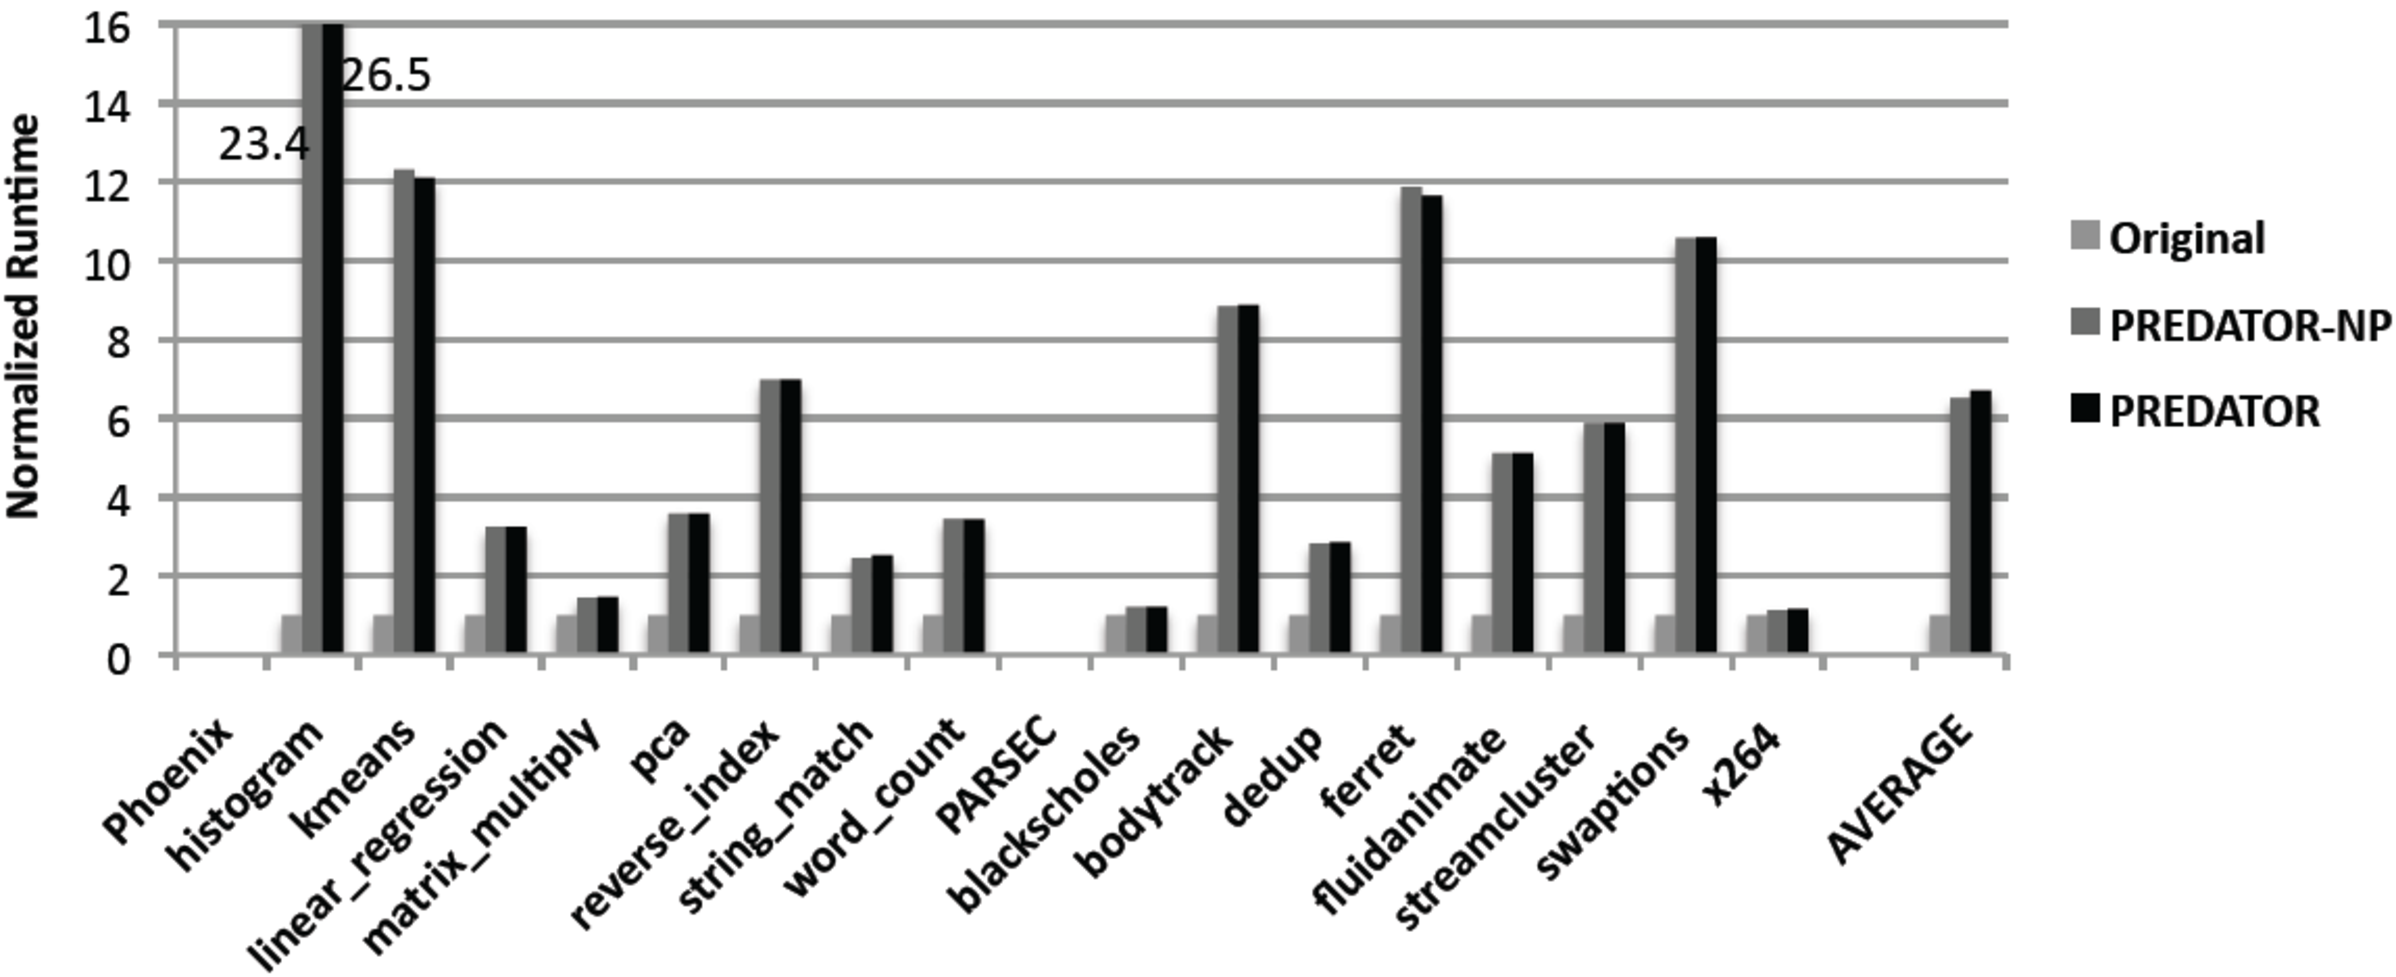
\includegraphics[width=5in]{fig/perf}
\end{center}
\caption{
Performance overhead of \defaults{} with and without prediction.
\label{fig:perf}}
\end{figure*}

Manifestness of false sharing highly depends on 

\subsection{Memory Overhead}
\label{sec:memoverhead}
Since \defaults{} pre-allocates a huge block of memory using \texttt{mmap} system call for 
its heap usage, 
virtual memory can not be used to tell actual memory overhead imposed by our tool. 
Hence, we only evaluate the physical memory overhead used by an application only. 
This number is based on proportional set size (PSS) in \texttt{/proc/self/smaps}
as discussed by Justin et al. ~\cite{memusage}. 

When evaluating an application, we start a script program to save 
corresponding \texttt{smaps} files periodically. 
The maximum number of total physical memory usage is selected for calculation.
%It is noted that we remove the physical memory usage of   
Results of memory usage is shown in Figure~\ref{fig:memusage}. As we can see,
\defaults{} does not increase memory usage substantially in all cases except for \texttt{swaptions}. 
Specifically, removing \texttt{swaptions} from calculation reduces 
the average memory overhead from 64\% to 22\%. 

The reason of \texttt{swaptions} using a large amount of memory is that 
its original memory usage is too small (only 3KB), and 
the additional memory added by \defaults{} in detection, prediction and
reporting yields a large number in percentage calculation. 

\begin{figure*}
\begin{center} 
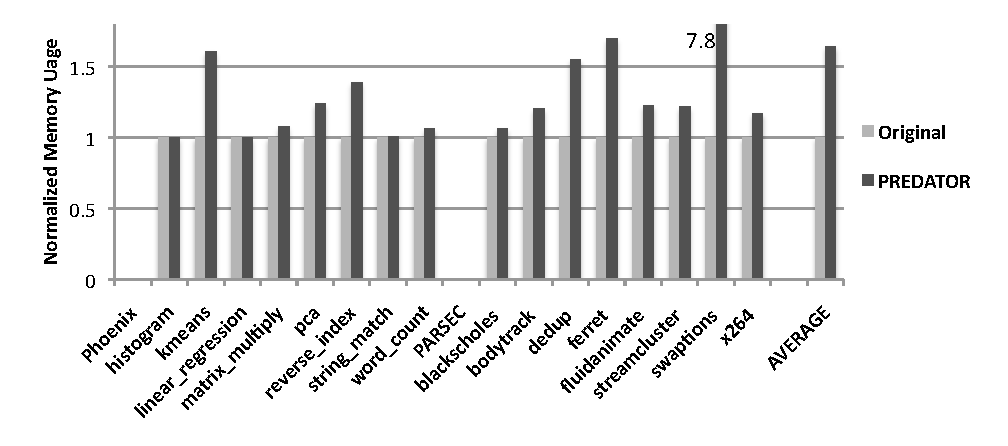
\includegraphics[width=5in]{fig/memusage}
\end{center}
%\includegraphics{fig/potential.pdf}
\caption{Memory usage overhead}
\label{fig:memusage}
\end{figure*}




\section{Related Work}
\label{sec:relatedwork}

This section describes related work in false sharing detection, prevention, or both; no prior work predicts false sharing.

\subsection{False Sharing Detection}
Schindewolf et al.\ designed a tool based on the SIMICS functional simulator to report different kinds of cache usage information, such as cache misses and cache invalidations~\cite{falseshare:simulator}. Pluto relies on the Valgrind dynamic instrumentation framework to track the sequence of memory read and write events on different threads, and reports a worst-case estimation of possible false sharing~\cite{falseshare:binaryinstrumentation1}.
Similarly, Liu uses Pin to collect memory access information, and reports total cache miss information~\cite{falseshare:binaryinstrumentation2}.
These tools impose about $100-200\times$ performance overhead.

Zhao et al.\ present a tool based on the DynamoRIO framework to detect false sharing and other cache contention problems
for multithreading programs~\cite{qinzhaodetection}. 
It uses a shadow memory technique to maintain memory access history and detects cache invalidations based on the ownership of cache lines. However, it can only support at most $8$ threads. In addition, it cannot differentiate cold cache misses from actual false sharing problems.

Intel's performance tuning utility (PTU) uses Precise Event Based Sampling (PEBS) hardware support to detect false sharing problems~\cite{detect:ptu,detect:intel}.  PTU cannot distinguish true sharing from false sharing. In addition, PTU aggregates memory accesses without considering memory reuse and access interleavings, leading to numerous false positives. Sanath et al.\ designed a machine learning based approach to detect false sharing problems. They train their classifier on mini-programs and apply this classifier to general programs~\cite{mldetect}. Instead of instrumenting memory accesses, this tool relies on hardware performance counters to collect memory accesses events. This approach operates with extremely low overhead but ties false sharing detection to a specific hardware platform.

In addition to their individual disadvantages,
all approaches discussed above share a common shortcoming:  
they cannot pinpoint the exact location of false sharing in the source code, so programmers must manually examine the source code to identify problems.

Pesterev et al.\ present DProf, a tool that help programmers identify cache misses based on AMD's instruction-based sampling hardware~\cite{DProf}. DProf requires manual annotation to locate data types and object fields, and cannot detect false sharing when multiple objects reside on the same cache line.

\subsection{False Sharing Prevention}

Jeremiassen and Eggers use a compiler transformation to automatically adjust the memory layout of applications through padding and alignment~cite{falseshare:compile}. Chow et al.\ alter parallel loop scheduling in order to avoid false
sharing~\cite{falseshare:schedule}. These approaches only works for regular, array-based scientific code.

Berger et al.\ describe Hoard, a scalable memory allocator that can reduce the possibility of false sharing by making different threads use different heaps~\cite{Hoard}. Hoard cannot avoid false sharing problem in global variables or within a single heap object: the latter appears to be the primary source of false sharing problems.

\subsection{False Sharing Detection and Prevention}

\sheriff{} provides two tools to handle false sharing based on its ``threads-as-processes'' framework~\cite{sheriff}.
\Sheriff{}'s detection tool reports false sharing accurately and precisely with only $20\%$ performance overhead.
However, it can only detect write-write false sharing, and only works for programs that use the \pthreads{} library. It can also break programs that communicate across different threads with stack variables or \emph{ad hoc} synchronizations. These shortcomings limit \Sheriff{}'s usefulness for real-world applications.  
\Predator{} can detect all kinds of false sharing and imposes no limitations on the kind of applications it works on. 

\Sheriff{}'s prevention tool prevents false sharing altogether, eliminating the need for programmer intervention. However, in programs with many synchronization calls, the overhead imposed by \Sheriff{} could lead to performance degradation.

Plastic leverages the sub-page granularity memory remapping facility provided by the Xen hypervisor to detect and tolerate false sharing automatically~\cite{OSdetection}. However, the sub-page memory remapping mechanism is not currently supported by most existing operating systems, reducing its generality. In addition, Plastic cannot pinpoint the exact source of false sharing.  
In order to utilize Plastic's prevention tool, a program has to run on the Xen hypervisor, limiting the applicability of their prevention technique.


\section{Future Work}
\label{sec:future}
\label{futurework}

We plan to extend \sheriff{} to find more performance related problems in
multithreaded programs. For example, if one frequently-read word
happens to be in the same cache line with one frequently-written word,
it would be better to separate those two words. But in the current
framework, \sheriff{} cannot detect a single memory read operation using the
twin page mechanism. We are examining the combination of hardware
watchpoints to help us locate this kind of performance error. In
addition, we plan to exploit watchpoints to capture those program
counters that touch specific addresses so as to point the programmer
to specific lines of code responsible for false sharing.



\label{sec:future}
\begin{comment}
(1) Pinpoint the line number to access the cache line by using the "watch point" technique. \\
(2) Figure out the problem caused by read-write false sharing problem by using the "watch point" technique. \\
(3) Design a run-time system which can tolerate the false sharing problem in a very low overhead. Profiling
on specified input should be very helpful to find the problem.
\end{comment}

\section{Conclusion}
This paper introduces \emph{evidence-based dynamic analysis}, a new
lightweight dynamic analysis technique. Evidence-based dynamic
analysis works for errors that can be forced to leave evidence of
their presence. These errors include key problems for C and C++
programs: buffer overflows, dangling-pointer errors, and memory
leaks. Evidence-based dynamic analysis is fast because it lets the
application run at full speed until an error is detected; execution is
then rolled back and replayed with instrumentation at the point where
the evidence was found, pinpointing the error. We
present \doubletake{}, the first evidence-based dynamic analysis
framework, and implement these analyses inside it. The resulting
analyses are the fastest versions to date, demonstrating the
effectiveness and efficiency of this new dynamic analysis approach.
\doubletake{} is available for download at \url{http://github.com/plasma-umass/DoubleTake}.


{
% \footnotesize
\small
\bibliographystyle{abbrv}
\bibliography{ref,emery}
}

\end{document}
